% vim: spell spelllang=en:
%! TEX root = **/00-main.tex

% Complete Data Mining process performed (one page, including a workflow).

\section{Data mining process}%
\label{sec:data_mining_process}

\begin{figure}[H]
    \centering
    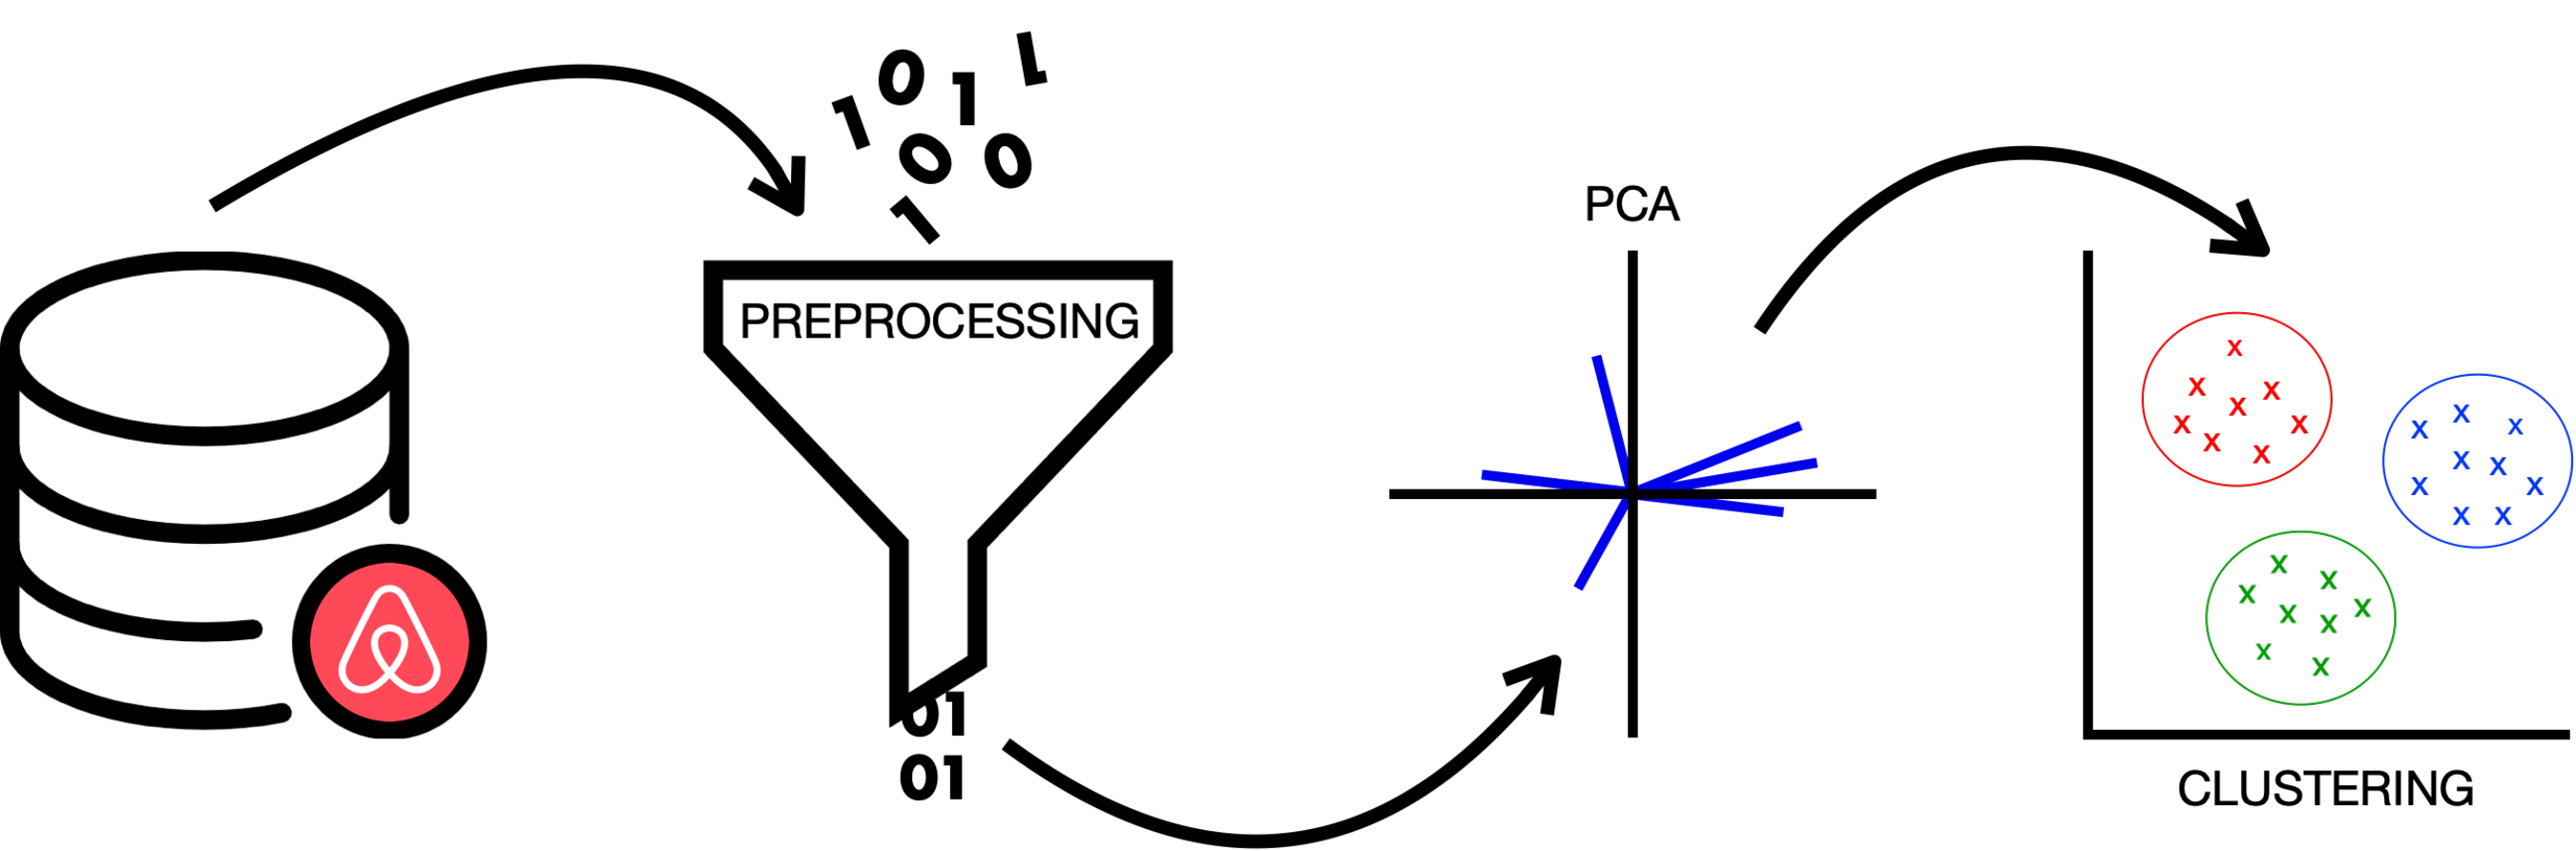
\includegraphics[width=0.6\linewidth]{images/workflow.pdf}
    \caption{Our data mining workflow}%
    \label{fig:airbnblistingsPlot.PNG}
\end{figure}

As discussed in \cref{sec:data_source}, our data came from a single dataset
in \emph{csv} format which we imported in R.

For the initial exploration, we imported the \emph{raw} dataset into R and
inspected the variables provided. Once we had a good understanding of the
variables, their meaning and how they were formated we proceeded with the
preprocessing of the data.

We made several decisions during the preprocessing which are explained in detail
in \cref{sec:preprocessing}. After preprocessing we had a reduced dataset with
a selection of the variables we deemed important for our study and without
any missing data.

From the preprocessed dataset we made a more formal statistical description of
the data: a univariate analysis for each variable and bivariate analysis of
various combinations of variables that seemed interesting.

% TODO el NA treatment al final el fem abans o despres de univariate?

The bivariate analysis gave us some insight into the relationships between the
different data columns which gave us some ideas of what to expect in the rest of
the exploratory steps.

For the PCA analysis we tried both the R built-in \texttt{prcomp} function and
the more feature-rich \texttt{PCA} provided by the \texttt{FactoMineR} library.
Although both gave the same results (except for some axis that where reversed),
the \texttt{FactoMineR} library provided more flexibility when representing data
so we used this one.

Similarly, we tried various methods and libraries for the hierarchical
clustering, which are explained in detail in its corresponding section.

\subsection{Workflow}%
\label{sub:workflow}

We decided to create an R script for each process (preprocessing, NA treatment,
PCA, clustering \dots). The data transformation scripts serialize the data frame
which is de-serialized in the other scripts. This makes it so that each script
can be executed independently of the rest without worrying about the current
environment (as long as there is the proper serialized file in the system).

To produce consistent plots we made all scripts share the same function to
export the plots to \emph{pdf} (see script in \cref{sub:shared.r}).

All the scripts used for the project are included in \cref{sec:r_scripts}.
